\documentclass[a4paper,10pt]{article}
\usepackage[utf8]{inputenc}

\usepackage[american]{babel}
\usepackage{graphicx}
\usepackage{amsmath}
\usepackage{amsthm}
\usepackage{amssymb}
%\usepackage{natbib}
\usepackage[margin=0.5in]{geometry}
\usepackage{fancyvrb}
\usepackage{pdfpages}
\usepackage{xcolor,colortbl, color}
\usepackage{lineno}
\usepackage{authblk}
\setlength{\parskip}{.1in}  
\setlength{\parindent}{0.0in}  
\linespread{1.6}
\usepackage[labelsep=period]{caption}

\setcounter{tocdepth}{1}
\setcounter{secnumdepth}{1}

\newcommand{\code}[1]{\texttt{#1}}

\begin{document}
\title{Experimental demonstration of an Allee effect in microbial populations}
\author[1*]{RajReni B. Kaul}
\author[1]{Andrew M. Kramer}
\author[2]{Fred Dobbs}
\author[1]{John M. Drake}

\affil[1]{Odum School of Ecology, University of Georgia, Athens, GA}
\affil[2]{Department of Ocean, Earth and Atmospheric Sciences, Old Dominion University, Norfolk, VA}
\affil[*]{\textit{corresponding author:} reni@uga.edu}
\date{}

\maketitle
%\textit{corresponding author}: RajReni B. Kaul reni@uga.edu


%\linenumbers
%\newpage


\section{Supplementary Material}
 
 \subsection{Methods}
\textit{Experimental Procedures}\\
The \textit{V. fischeri} strain ES114 containing the naturally occurring plasmid pVSV102 altered to carry a constitutively expressed green fluorescence protein (GFP) and kanamycin-resistance cassettes was used in all experiments \cite{dunn_new_2006}.  \textit{V. fisheri} strain ES114 pVSV102 and \textit{C. roenbergensis} were kindly supplied by Eric Stabb (UGA) and Alexander Bochdansky (ODU), respectively. 
 
 All populations were grown in mineral salts medium (0.4mM NaPO$_{4}$ (pH 7.5), 50mM Tris (pH 8.0), 11mM NH$_{4}$Cl, 10$\mu$M  FeSO$_{4}\cdot$7H$_{2}$O, 55mM MgSO$_{4}\cdot$7H$_{2}$O, 11mM KCl, 0.3M NaCl, 11mM CaCl$_{2}\cdot$2H$_{2}$O) containing 20 mM glycerol under kanamycin selection (100mg/mL). The high carbon resource environment had an additional 20mM glycerol. 

Individual cells of \textit{V. fischeri} and \textit{C. roenbergensis} were selected to inoculate experimental populations by fluorescence flow sorting (MoFlo XDP Beckman Coulter, Hialeah, Florida ). Exponential phase cultures of \textit{V. fischeri} and \textit{C. roenbergensis} were stained with 3$\mu$M propidium iodide (PI), a membrane impermeable nucleic acid dye, for 15 minutes prior to sorting into  microplate wells holding appropriate media. This method allowed populations to be accurately initiated with geometrically increasing number of viable cells (1 to 64 cells in high resource and 1 to 2048 cells in low resource). The high carbon resource experiment was conducted in 3 replicate 96 well microplates with  each well having a final volume of 200$\mu$L. The low carbon resource experiment was done in a 384 well microplate with a final well volume of 75$\mu$L. The switch to a higher well plate allowed for a paired control and treatment experimental design within a single plate. The volume difference created non-identical but overlapping density treatments of 5, 10, 20, 40, 80, 160 and 320 $cells~mL^{-1}$ for the higher carbon resource treatment ($n=36$ wells per density) and  13 , 27 , 53 , 107 , 213 , 427 , 853 , 1 707 , 3 413 , 6 827 , 13 653 , and 27 307 $cells~mL^{-1}$ for the low resource treatment ($n=24$). Ten \textit{C. roenbergensis} per population ($133~cells~mL^{-1}$)  were added to half of the low resource treatment replicates ($n=12$ wells per density with and without predation). The \textit{HC} treatment was toxic to \textit{C. roenbergensis}, so these populations were not exposed to predation.  


Immediately following well inoculation, the microtiter plates were sealed with optical film to avoid contamination. Plates were simultaneously incubated at $28\,^{\circ}\mathrm{C}$ and monitored for growth based on optical density (OD$_{620}$) and GFP fluorescence (485/528, sensitivity=100) in a Synergy H1 plate reader (Biotek). Populations were allowed to grow for 96 hours before assessing population establishment. Established populations, scored as 1, were defined as having an increase of at least 0.25 OD$_{620}$ or 100 relative fluorescence units (RFUs) from the initial reading. The threshold used ensured that noise inherent in the plate reader would not be considered growth. 

\textit{Model Fitting}\\
The presence of an Allee effect was separated from stochastic variation by estimating the probability of establishment as a function of initial population density. The stochastic theory of subcritical population growth entails that the probability of small populations establishing when regulated by an Allee effect will accelerate (positive second derivative) with respect to initial population size \cite{dennis_allee_2002}. The probability of establishment will decelerate (negative second derivative) with respect to initial population size once the population is large enough to escape the Allee effect. This switch between accelerating and decelerating probability, or inflection point occurs at the minimum density needed to escape an Allee effect.  This value is also known as the critical threshold. If stochasticity alone determines population establishment, the relationship between probability of establishment and population size is strictly monotonic.   For this reason, we chose a function that can be either monotonic or sigmoidal depending on parameterization. The 2-parameter Weibull function is flexible,

\begin{equation}
 p = 1-e^{(\frac{-x}{\lambda})^{k}},
\end{equation}

\noindent where $p$ is the probability of establishment, $x$ is the $\ln \text{(initial population density}~(cells~mL^{-1}))$, $k$ dictates the shape (monotonic or sigmoidal), while $\lambda$ influences the scale.  Conveniently, the function is undefined at $x< 0$ (negative initial population sizes). When the 2-parameter Weibull function is sigmoidal (shape parameter, $k>1$), the maximum of the second derivative or inflection point  is,
\begin{equation}
       \tilde x = \lambda \left(\sqrt[k]{\frac{k-1}{k}}\right),
\end{equation}

and the limit of the expression as $k$ approaches infinity is $\lambda$.  Therefore the possible value of the inflection point or critical population size needed to escape an Allee effect must fall between 1 and $\lambda$. The mean probability of establishment is bounded $(0,1)$ and therefor violates assumptions of normality. For this reason, we use the binary outcome of each population for data analysis assuming a binomial distribution. 
%Binomial likelihood
Interpreting this model as the mean outcome of independent trials gives rise to a binomial distribution with the following likelihood,

\begin{equation}
L(p)= L(y|p)= p^{y} (1-p)^{(n-y)},
\end{equation}

\noindent where $y$ is the total number of established populations in $n$ populations. The parameters $k$ and $\lambda$ were simultaneously fit using maximum likelihood via simulated-annealing \cite{bbmlepack, baseR}. Initial parameter values were set to one.  The 95\% confidence intervals were determined from the likelihood surface calculated during the fitting process assuming a $\chi^{2}$ distribution.  The threshold value used for hypothesis testing is $k=1$, above or below this value the Weibull is sigmoidal or inverse exponential decay, respectively.
 The null hypothesis of no Allee effect was rejected if the estimated confidence interval of the shape parameter $k$ did not include $k<1$.

\textit{Sensitivity Analysis}

To investigate the robustness of our conclusions, we tested for the effect of any high leverage observations using a point-wise drop scheme in which each observation was removed from the data before calculating the parameter point estimate and likelihood surface. This procedure was repeated until all points had been omitted from analysis.  If the analysis was sensitive to any particular observation, removal would result in a dramatic change of the likelihood surface and the location to the 95\% confidence interval with respect to $k=1$. 

\subsection{Results}

Prior to inoculation into microplate wells, roughly 90\% of the \textit{V. fischeri} culture met the viable cell criteria set by the flow cytometer. The yield, or carrying capacity, of an experimental population was not significantly correlated with density treatment in the high resource environments ($R^{2}=$7e-04, $p=$0.686). The yield in low resource environments was significant but weakly correlated with density treatment ($R^{2}=$0.09, $p=$0.000418, $R^{2}=$0.2, $p=$3.35e-06; without and with predation). The proportion of populations establishing increased and time to detection decreased non-linearly with initial density, indicating reduced growth rate at low density populations (Table 1). In the \textit{HC} environment estimated parameters were $\hat k=2.57$ (95\% CI (1.72,3.65)) and $\hat \lambda=1.92$ (95\% CI (1.64, 2.12)). The estimated shape and scale parameters were larger in the \textit{LC} environment, $\hat k=11.7$ (95\% CI (5.42, 24.2)), and $\hat \lambda=3.19$ (95\% CI (3.01, 3.43)). The Weibull shape parameter of the \textit{LCP} treatment was in between, $\hat k=5.8$ (95\% CI (3.78, 8.75)), while the scale parameter continued to increase, $\hat \lambda=4.64$ (95\% CI (4.33, 4.99)). 

The likelihood surfaces from the sensitivity analysis were overlaid to create a cloud of confidence intervals (Figure S1). While there was minor deviations from the fit calculated from the complete data set, no deviation would lead us to fail to reject the hypothesis. This analysis shows the experiment included an adequate number of replicates and our overall conclusion are robust.

\subsection{Applications}

Impacts of Allee effects extend far beyond marine bacteria to the dispersal of all microbes \cite{litchman_invisible_2010} including those associated with disease. For example, the infectious dose response curve used to quantify the rate of infection given a pathogen inoculum size is often sigmoidal, possibly indicating an Allee effect. When such a response is incorporated into host-parasitoid models the threshold for successful parasitoid invasion is substantially higher than the standard models \cite{regoes_dose-dependent_2002}.  Another related pattern is the \textit{in vitro} propagation of human cancer cells, which has a high failure rate when inoculated with very low cell densities \cite{axelrod_evolution_2006}. This  result implies that positive density dependence of microbial populations (or, in the case of cancer, subclones) may  also influence development of successful therapeutic treatments \cite{korolev_turning_2014}.
   
By affecting trophic interactions of the microbial loop, predator-induced demographic Allee effects could alter efficacy of biotechnological processes. The use of predation as a microbial biocontrol is promising for controlling seafood-borne illnesses. For instance, predation by \textit{Bdellovibrio} and like organisms (BALOs) mitigates uptake and persistence of pathogenic \textit{Vibrios} in Eastern oysters (\textit{Crassostrea virginica}) \cite{richards_predatory_2012}. Altering the microbial loop via bacterial predation in some systems increases bioremediation rates through non-consumptive effects of the predator, while in other systems predation reduces the bacterial load dramatically, dampening contaminant breakdown (as reviewed in \cite{saleem_multitrophic_2014}). Microbial predation has been proposed as a tool in other biotechnology settings, including facilitating nutrient cycling and plant growth in addition to waste water treatment. Regardless of the system, a predator-induced extrinsic demographic Allee effect could enhance or inhibit microbial action depending on the intended outcome. Further work along these lines could be used to additionally develop long standing microbial concepts such as quorum protection \cite{macreadie_quorum_2015} and minimum inhibitory concentration \cite{steels_sorbic_2000} in addition to burgeoning biotechnological applications of microbial predation. 

%\section{References}
%\bibliographystyle{plain}%Choose a bibliograhpic style
\bibliographystyle{biologyletters}
\bibliography{MS_supp}

\newpage
\renewcommand{\figurename}{Figure S}

\section{Figures}
\begin{figure}[!h]
\begin{center}
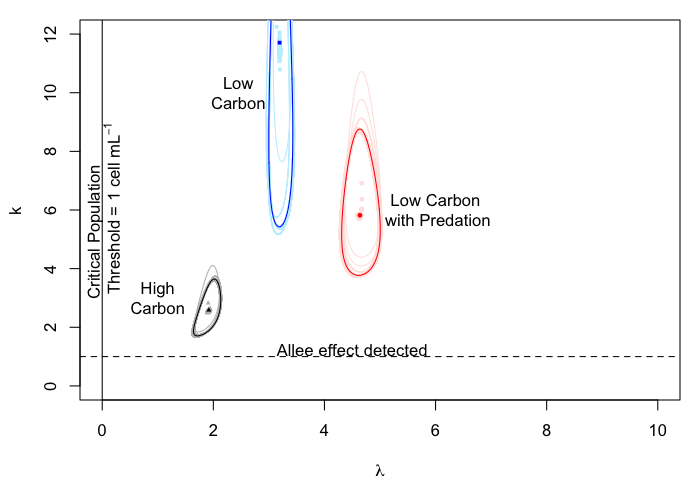
\includegraphics[width=\textwidth]{pointwise.png}
\end{center}
\caption{\textbf{Sensitivity Analysis.} The point estimate and 95\% confidence interval were estimated from the full dataset ($n$ observations in bold). The analysis was repeated with $n-1$ observations until each case had individually been omitted (pale color). Removal of a single observation does not impact Allee effect detection indicating the robustness of conclusion. }


\end{figure}

\end{document}